\section{Evaluation}
\label{sec:evaluation}

This section evaluates FeBEx using a Mininet-based BMv2 testbed and a Python P4Runtime controller. Our goal is to quantify how effectively FeBEx reduces redundant backhaul traffic while preserving correct delivery, tenant isolation, and attribution semantics. We additionally study the effect of key design parameters, including register size, epoch interval, and switch variant.

\fakepar{Evaluation Setup}
We evaluate FeBEx on Mininet with BMv2 and a Python P4Runtime controller. The topology contains $K$ gateway hosts generating packet copies according to a coverage matrix, one FeBEx BMv2 switch, $M$ tenant LNS hosts, and one cloud host receiving cloned receipts. Traffic generation, packet capture, and metric computation are automated end-to-end. For each experiment point, we run both a \textit{Dedup OFF} baseline, in which the switch performs only routing, and a \textit{Dedup ON} mode, in which FeBEx actively suppresses duplicates.

\fakepar{Metrics}
We report five primary metrics. \textit{Backhaul savings} is computed as$1 - \frac{\text{packets}_{\text{ON}}}{\text{packets}_{\text{OFF}}},$
capturing the fraction of redundant traffic eliminated by FeBEx. \textit{Delivery ratio} measures the fraction of unique uplinks that are correctly received at the intended tenant backend. \textit{Tenant isolation} counts any cross-tenant forwarding violations. \textit{Duplicate leakage} measures the number of duplicate packets that still pass through under deduplication. Finally, \textit{throughput} is measured as the effective packet rate observed at the receiver.


\fakepar{Experiment Matrix}
Our evaluation covers eight experiment families. E1 measures backhaul savings as a function of duplicate factor. E2 evaluates correctness through the delivery ratio of unique uplinks. E3 checks multi-tenant isolation. E4 studies scalability across increasing numbers of devices and gateways. E5 sweeps register size to understand state-provisioning tradeoffs. E6 sweeps epoch interval to evaluate temporal sensitivity. E7 verifies correctness of cloned payment receipts and gateway attribution. E8 compares the three switch variants V1, V2, and V3 under boundary and collision stress.

\fakepar{Configuration}
Unless otherwise stated, experiments use a medium-city configuration with 100 devices, 10 gateways, and 4 tenants, together with fixed random seeds for reproducibility. Register size and epoch interval are swept only in E5 and E6, respectively. For E8, we keep the workload and topology fixed and vary only the switch variant so that differences can be attributed to the deduplication design itself.
\begin{figure}[t]
\centering
\resizebox{0.95\linewidth}{!}{%
\begin{tikzpicture}[node distance=5mm and 5mm]
\node[block] (cov) {Generate coverage\\and tenant map};
\node[block, right=of cov] (start) {Start topology,\\receivers, controller};
\node[block, right=of start] (run) {Run gateway\\traffic};
\node[block, right=of run] (collect) {Collect LNS\\and cloud logs};
\node[block, right=of collect] (metrics) {Compute metrics\\and plots};

\draw[line] (cov) -- (start);
\draw[line] (start) -- (run);
\draw[line] (run) -- (collect);
\draw[line] (collect) -- (metrics);
\end{tikzpicture}%
}
\caption{\emph{End-to-end evaluation workflow.} Each experiment run generates the workload, executes the FeBEx topology, collects outputs from tenant and cloud endpoints, and computes the reported metrics.}
\label{fig:eval-workflow}
\end{figure}
% \begin{figure}[t]
% \centering
% \fbox{\parbox{0.95\linewidth}{
% \textbf{Evaluation Workflow}\\[1mm]
% Generate coverage + tenant mapping\\
% $\downarrow$\\
% Start topology, receivers, and controller\\
% $\downarrow$\\
% Run gateway traffic generators\\
% $\downarrow$\\
% Collect LNS/cloud logs\\
% $\downarrow$\\
% Compute metrics and render plots
% }}
% \caption{\emph{End-to-end workflow used in every experiment run.}}
% \label{fig:eval-workflow}
% \end{figure}


\fakepar{E1: Backhaul Savings}
Figure~\ref{fig:e1-backhaul} shows the backhaul savings achieved by FeBEx as the duplicate factor increases. FeBEx provides strong bandwidth reduction, with savings rising from low-duplication scenarios to high-duplication scenarios, closely matching the expected trend. Savings increase from approximately 25\% at low duplication to about 86\% at high duplication, approaching the theoretical limit as more gateways hear the same uplink. Minor deviation at the highest stress point is consistent with BMv2 software effects under load rather than instability in the deduplication logic. Overall, these results show that in-network deduplication provides predictable and substantial backhaul reduction, with the largest gains in dense multi-gateway coverage regions.

\begin{figure}[t]
    \centering
    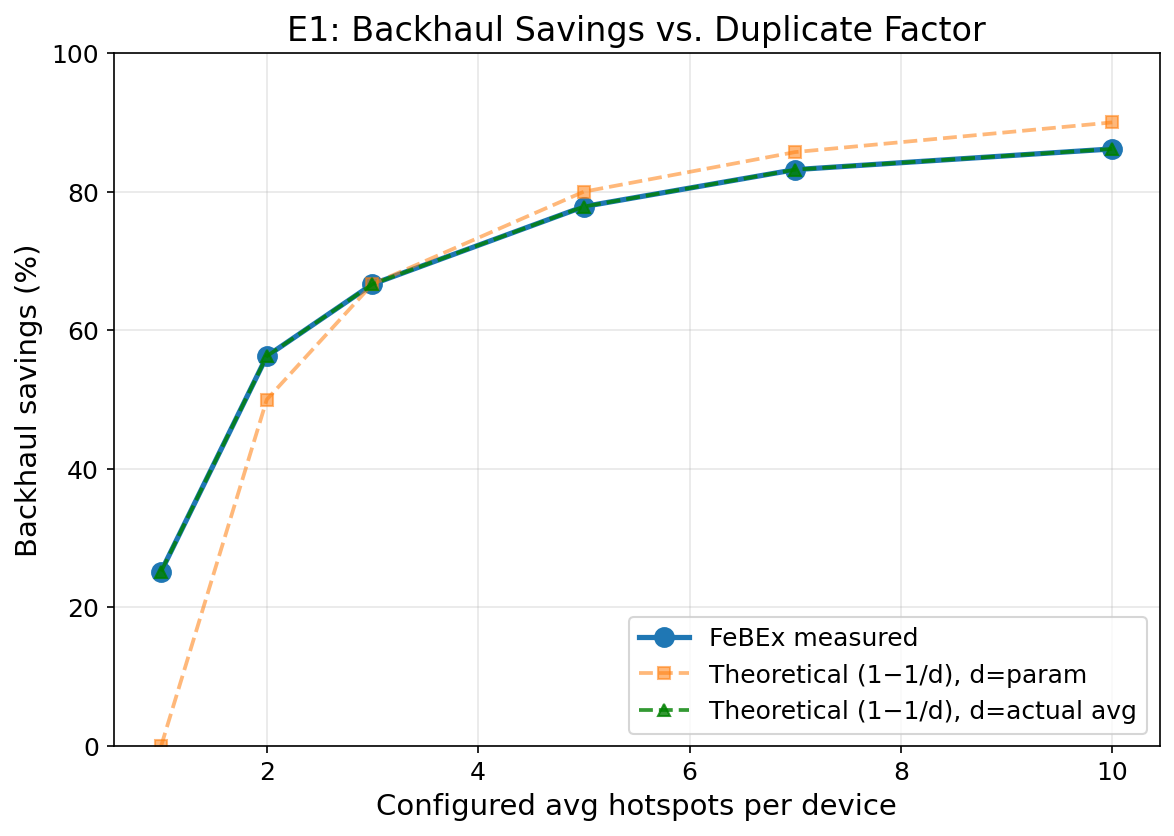
\includegraphics[width=0.5\linewidth]{figures/E1_backhaul_savings.png}
    \caption{\emph{Backhaul savings versus duplicate factor.} Savings increase with duplication and approach the theoretical limit as more redundant gateway copies are suppressed in-network.}
    \label{fig:e1-backhaul}
\end{figure}

\fakepar{E2: Correctness and Delivery Ratio}
Figure~\ref{fig:e2-correctness} plots the delivery ratio of unique uplinks under deduplication. Delivery remains effectively perfect for normal operating points, and degradation appears only under extreme offered load where BMv2 software limitations dominate. In realistic and moderate-duplication settings, the delivery ratio remains approximately 1.0, indicating that FeBEx does not falsely suppress legitimate first copies. The small drop observed only at the most stressful operating point is consistent with software-switch bottlenecks rather than a flaw in the deduplication design. These results indicate that FeBEx preserves correctness across realistic operating ranges.

\begin{figure}[t]
    \centering
    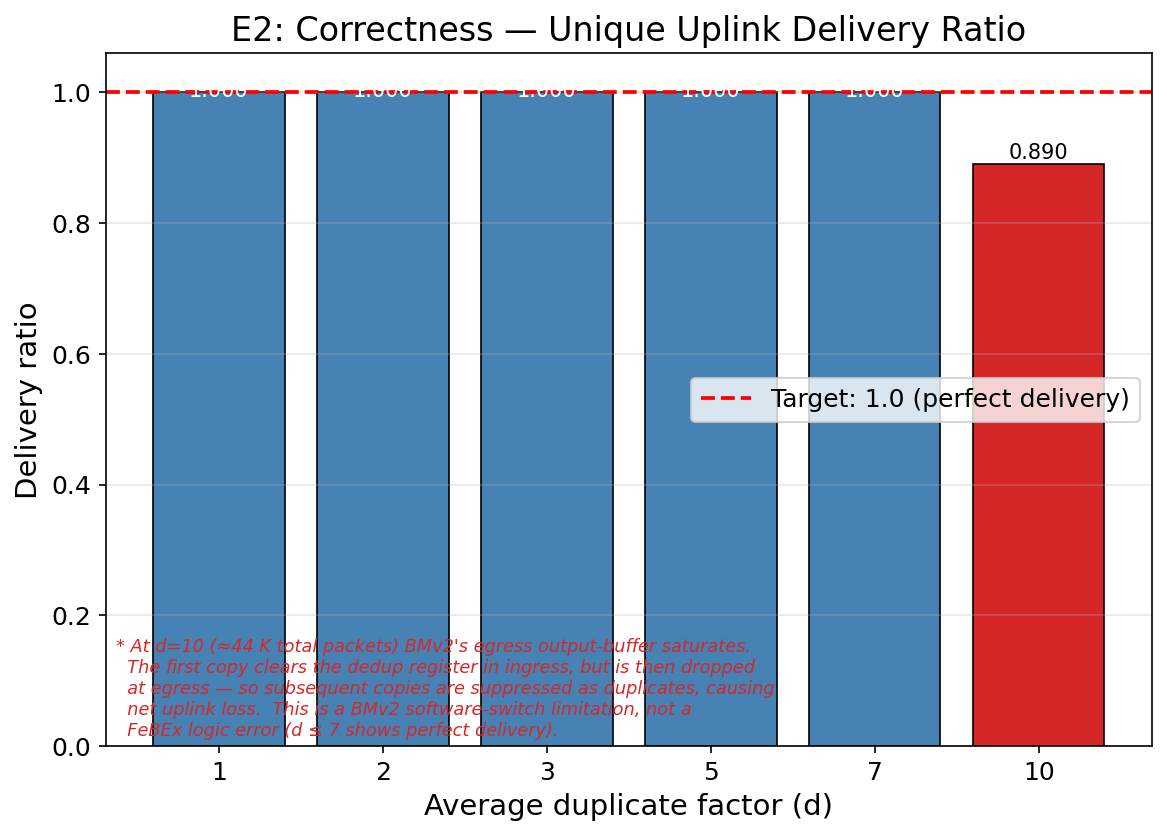
\includegraphics[width=0.5\linewidth]{figures/E2_correctness.png}
    \caption{\emph{Delivery ratio of unique uplinks under deduplication.} FeBEx maintains near-perfect correctness across normal operating points, with degradation only under extreme software-switch stress.}
    \label{fig:e2-correctness}
\end{figure}


\fakepar{E3: Multi-Tenant Isolation}
We next evaluate whether FeBEx preserves tenant boundaries while suppressing duplicates. Across the tested four-tenant scenario and thousands of forwarded packets, we observe no cross-tenant delivery violations. DevAddr-prefix-based LPM steering remains consistent under both routing-only and dedup-enabled modes. This confirms that duplicate suppression does not interfere with multi-tenant forwarding correctness, and that FeBEx can be deployed without breaking tenant isolation.

\fakepar{E4: City-Scale Scalability}
Figure~\ref{fig:e4-scalability} evaluates FeBEx across increasing deployment sizes. Across small, medium, and large scenarios, FeBEx maintains substantial backhaul savings while throughput trends are dominated by software-switch capacity rather than algorithmic instability. Savings remain in a similar range, roughly from the high-50s to the high-60s percent, even as topology size increases from small to city-scale settings. Throughput rises initially and then drops at the largest emulation size, indicating saturation effects in BMv2 and Mininet. Thus, the deduplication behavior itself scales stably with topology growth, while the throughput ceiling is primarily an artifact of the software target.

\begin{figure}[t]
    \centering
    
\includegraphics[width=0.9\linewidth]{figures/E4_scalability.png}
    \caption{\emph{Scalability across deployment sizes.} FeBEx maintains substantial backhaul savings as the number of devices and gateways increases, while throughput trends mainly reflect software-switch limits.}
    \label{fig:e4-scalability}
\end{figure}

\fakepar{E5: Register Sizing Sensitivity}
Figure~\ref{fig:e5-sizing} studies the effect of register size on duplicate leakage and savings. As expected, larger register arrays sharply reduce collision-driven leakage. The largest improvement occurs when moving from very small tables to moderately sized ones, for example from 256 to 1024 entries, after which the benefit begins to plateau. Beyond 4096 entries, additional memory yields only diminishing returns for the evaluated workloads. Savings follow the same trend. These results support a practical rule of thumb for FeBEx deployment: provision register capacity at no less than $4\times$ the expected active device count.

\begin{figure}[t]
    \centering
    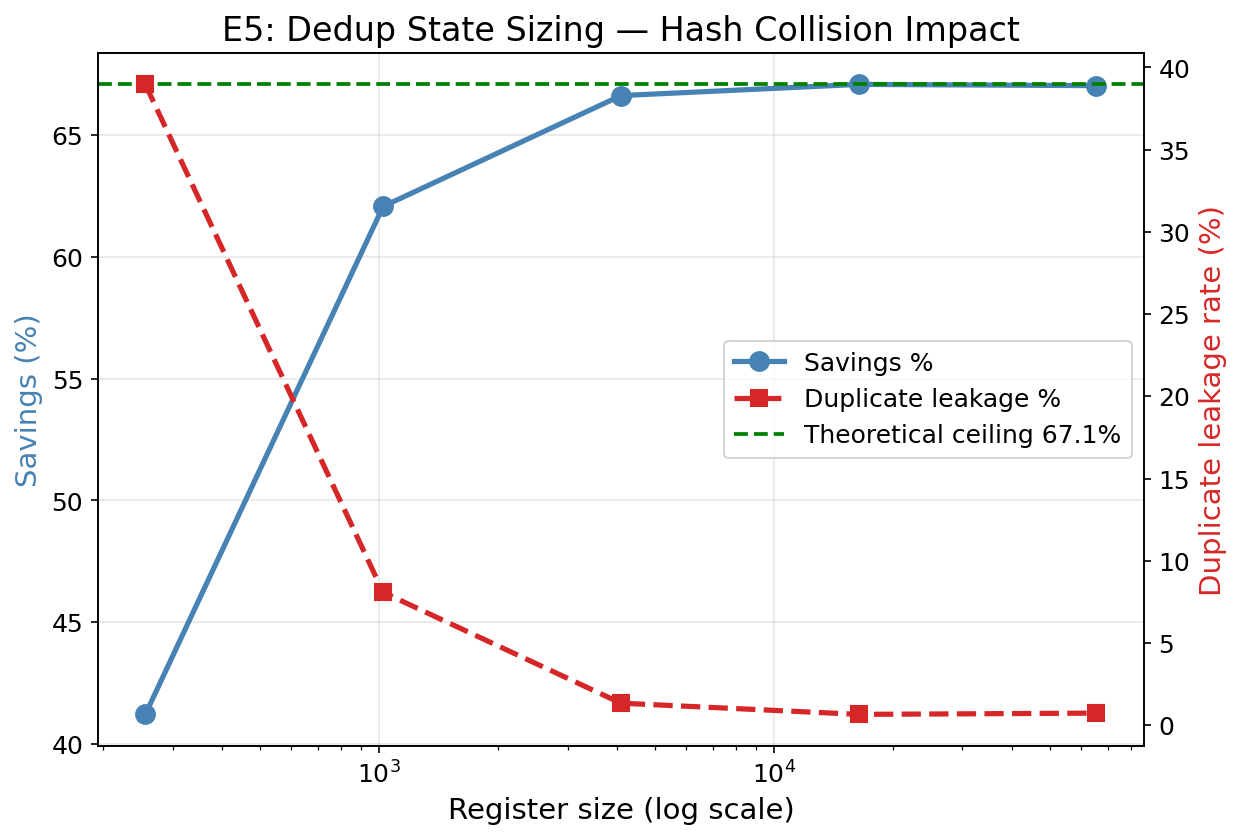
\includegraphics[width=0.5\linewidth]{figures/E5_state_sizing.png}
    \caption{\emph{Effect of register size on deduplication performance.} Larger register arrays sharply reduce duplicate leakage and improve backhaul savings, with diminishing returns beyond moderate table sizes.}
    \label{fig:e5-sizing}
\end{figure}



\fakepar{E6: Epoch Interval Sensitivity}
Figure~\ref{fig:e6-epoch} evaluates the impact of epoch interval on deduplication effectiveness. Very short epochs increase boundary leakage because repeated packets are more likely to straddle an epoch transition, while moderate epoch intervals provide stable suppression with minimal stale-state effects. In our experiments, leakage decreases monotonically as the epoch interval increases, with near-zero leakage observed at 10 seconds and above. Extremely aggressive intervals, such as sub-second or 1-second rotations, amplify boundary effects significantly. These results suggest that FeBEx should avoid overly short epochs; intervals of 5--10 seconds provide a robust operating region for the workloads considered here.

\begin{figure}[t]
    \centering
    
\includegraphics[width=0.5\linewidth]{figures/E6_epoch_sensitivity.png}
    \caption{\emph{Impact of epoch interval on deduplication effectiveness.} Moderate intervals reduce boundary leakage while maintaining simple, bounded-state expiry.}
    \label{fig:e6-epoch}
\end{figure}

\fakepar{E7: Payment Receipt Attribution}
We next verify that FeBEx preserves attribution semantics alongside duplicate suppression. Across the evaluated scenarios, cloned cloud receipts maintain a one-to-one correspondence with the first-forwarded tenant packets, and the gateway identifiers embedded in those cloned packets remain valid. This confirms that FeBEx does not merely suppress duplicates correctly, but also preserves the receipt semantics needed for Proof-of-Coverage and payment-related accounting.

\fakepar{E8: Variant Comparison}
Figure~\ref{fig:e8-variant} compares the three FeBEx switch variants under boundary-stress settings. V2, which uses a sliding-window check over the current and previous epoch, exhibits the best behavior when boundary leakage is the dominant source of error, since it suppresses duplicates that straddle an epoch transition. V3 improves collision-oriented behavior through its dual-register Bloom-style design, but it does not eliminate boundary leakage by itself, and therefore remains below V2 on this stress case. V1, as the baseline, is most exposed to cross-boundary duplicate leakage. These results suggest a clear deployment guideline: use V2 when boundary leakage is expected to dominate, and treat V3 as a complementary design for collision robustness rather than a direct solution to epoch-boundary effects.

\begin{figure}[t]
    \centering
    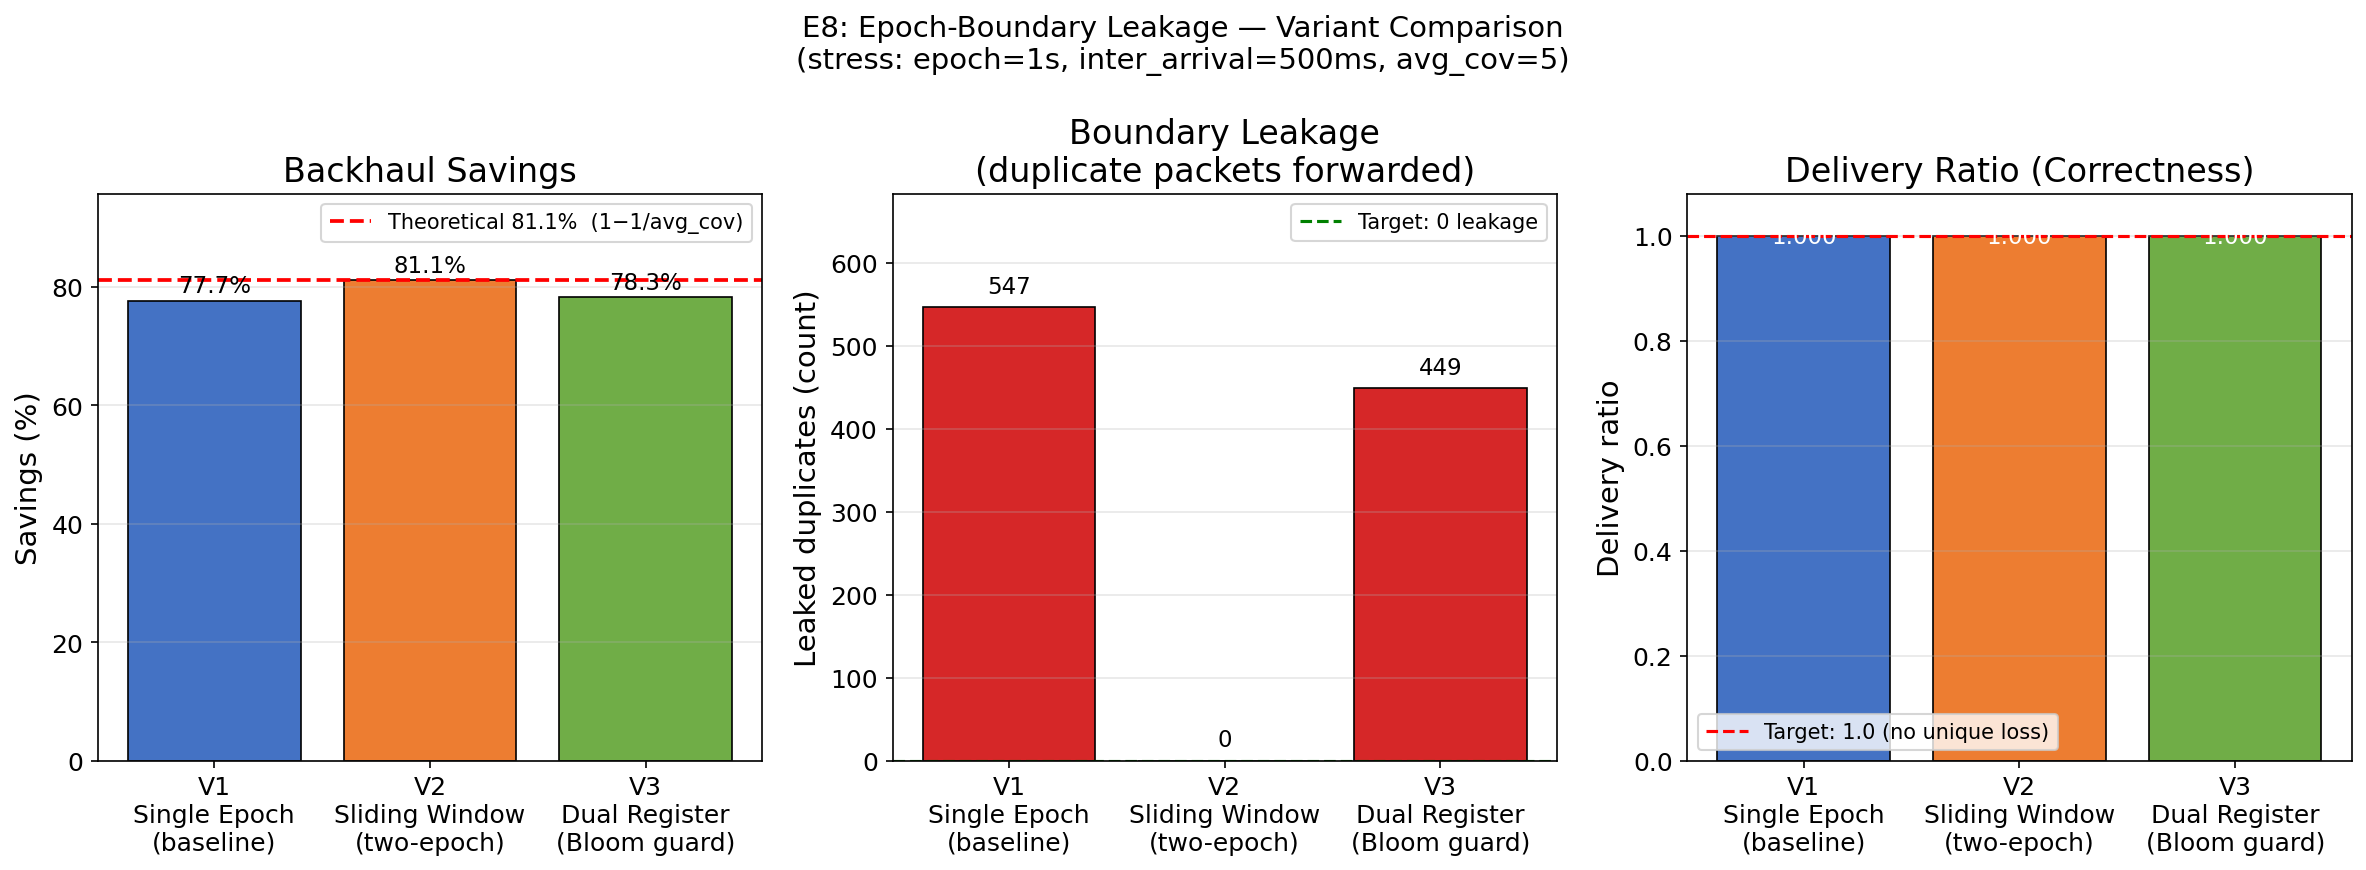
\includegraphics[width=\linewidth]{figures/E8_variant_comparison.png}
    \caption{\emph{Variant comparison under boundary stress.} V2 provides the strongest suppression of cross-boundary duplicates, while V3 primarily improves collision behavior rather than boundary robustness.}
    \label{fig:e8-variant}
\end{figure}

\fakepar{Threats to Validity}
Our evaluation has three main limitations. First, BMv2 is a software target and can saturate under high offered load, so absolute throughput numbers should not be interpreted as hardware dataplane limits. Second, the packet format is intentionally simplified to isolate the backhaul deduplication problem rather than emulate a full LoRaWAN parsing pipeline. Third, our results emphasize the behavior of the deduplication logic and the resulting design trends, rather than the exact performance of a production hardware switch.

\fakepar{Evaluation Summary}
Overall, the experiments show that FeBEx consistently reduces backhaul traffic, preserves correctness and tenant isolation, and maintains attribution semantics required for Helium-style deployments. The results also expose clear operational tuning knobs: register size controls collision-induced leakage, epoch interval governs temporal boundary effects, and the choice of switch variant determines whether the design prioritizes boundary robustness or collision resistance.